% ---------------------------------------------------------------------
% Appendix A.1: Rust DSVH pseudocode
% ---------------------------------------------------------------------
\setcounter{section}{14}
\subsection{Appendix A.1: Rust --- Deterministic Sovereign Vector Heap (DSVH)}
\label{app:rust-dsvh}

The Deterministic Sovereign Vector Heap (DSVH) is the production
implementation of the FNV-1a signed-hash projection formalized in
\S\ref{sec:formalization}. The DSVH is implemented in Rust because
the dominant invariant is \emph{bitwise determinism under concurrent
readers}: every corpus scan must produce the same byte sequence
regardless of which thread executes the scan. This appendix
documents the DSVH at the level of academic pseudocode; the
production source is bitwise-equivalent to the pseudocode below
modulo the borrow-checker and lifetime annotations.

\subsubsection{Type Definitions}

The DSVH is built on four core types. The types are designed for
cache-line alignment and zero-copy serialization.

\begin{algorithm}[t]
\caption{DSVH Type Definitions}
\label{alg:dsvh-types}
\SetAlgoNoLine
\BlankLine
\KwData{$\mathbb{V}$ = projection dimension ($D = 128$)}
\BlankLine
$\mathbf{type}\ \mathit{Vector} \in \mathbb{R}^{\mathbb{V}}$\;
$\mathbf{type}\ \mathit{TokenStream} = \mathbf{Seq}[\mathit{Token}]$\;
$\mathbf{type}\ \mathit{Projector} = \mathbf{String} \to \mathit{Vector}$\;
$\mathbf{type}\ \mathit{Heap} = \mathbf{Arc}[\mathbf{RwLock}[\mathbf{HashMap}[\mathit{Vector}, \mathit{DocumentID}]]]$\;
\BlankLine
\textbf{Invariant} ($\mathbf{Heap\ Invariant}$): \tcp*{deterministic read-only}
The DSVH heap is read-heavy: every operation is either a
$\mathbf{Query}(q)$ that returns the top-$k$ documents by cosine
similarity, or an $\mathbf{Insert}(d, v)$ that adds a new document
with its pre-computed vector. The dominant invariant is that
$\mathbf{Query}(q)$ is \emph{wait-free} for concurrent readers and
returns byte-identical results regardless of which thread executes
the query.
\end{algorithm}

\subsubsection{The FNV-1a Projection Pipeline}

The DSVH implements the four-formula stack of \S\ref{sec:formalization}
as a five-stage pipeline. The pipeline is documented as an
\texttt{algorithm2e} block below.

\begin{algorithm}[t]
\caption{DSVH FNV-1a Projection Pipeline}
\label{alg:dsvh-pipeline}
\SetAlgoLined
\KwIn{Document $d \in \mathbf{String}$, projection dimension $D = 128$,
bigram seed $\sigma_b = 1$, unigram seed $\sigma_u = 2$, FNV prime
$p = 0x100000001b3$, offset basis $b_0 = 0xcbf29ce484222325$}
\KwOut{Normalized vector $v \in \mathbb{R}^{128}$ with $\|v\|_2 = 1$}
\BlankLine
$\mathit{tokens} \gets \mathrm{TOKENIZE}(d)$ \tcp*{unigrams + bigrams, length $\ge 2$}
$v \gets \mathbf{zeros}[D]$\;
\ForEach{$t \in \mathit{tokens}$}{
  $h \gets \mathrm{FNV1a}(t, \sigma)$ \tcp*{$\sigma \in \{\sigma_b, \sigma_u\}$}
  $k \gets h \bmod D$\;
  $\xi \gets 1 - 2(h \mathbin{\&} 1)$ \tcp*{Rademacher sign}
  $v[k] \gets v[k] + \xi$\;
}
$\|v\|_2 \gets \sqrt{\sum_{k=0}^{D-1} v[k]^2}$\;
\If{$\|v\|_2 > 0$}{
  \For{$k \gets 0$ \KwTo $D - 1$}{
    $v[k] \gets v[k] / \|v\|_2$ \tcp*{$L_2$ spherical normalization}
  }
}
\KwRet $v$\;
\caption*{The four-formula projection pipeline:
\texttt{TOKENIZE} $\to$ \texttt{FNV1a} $\to$ sign extraction $\to$
$L_2$ normalization. The pipeline produces the normalized vector
$v \in S^{127}$ that is the canonical input to the cosine similarity
ranking of \texttt{Query}.}
\end{algorithm}

\subsubsection{Query and Cosine Similarity}

The DSVH query operation scans the heap and returns the top-$k$
documents by cosine similarity. The scan is wait-free for concurrent
readers and uses the cosine-equals-dot-on-the-unit-hypersphere
equivalence of Theorem~\ref{thm:cosine-dot}.

\begin{algorithm}[t]
\caption{DSVH Query (Top-$k$ Cosine Similarity)}
\label{alg:dsvh-query}
\SetAlgoLined
\KwIn{Query vector $q \in S^{127}$, heap $\mathcal{H}$, top-$k$
parameter $k$}
\KwOut{Top-$k$ documents $\{(d_i, s_i)\}_{i=1}^{k}$ sorted by
$s_i = q \cdot v_i$ in descending order}
\BlankLine
$\mathcal{R} \gets \mathbf{PriorityQueue}[(\mathbf{DocumentID}, \mathbb{R})]$\;
$\mathbf{read\_lock}(\mathcal{H})$ \tcp*{wait-free read}
\ForEach{$(d, v) \in \mathcal{H}$}{
  $s \gets q \cdot v$ \tcp*{dot product on the unit hypersphere}
  $\mathcal{R}.\mathbf{push}(d, s)$\;
  \If{$\mathcal{R}.\mathbf{size} > k$}{
    $\mathcal{R}.\mathbf{pop\_min}()$ \tcp*{maintain top-$k$}
  }
}
$\mathbf{read\_unlock}(\mathcal{H})$\;
\KwRet $\mathcal{R}.\mathbf{sort\_descending}()$\;
\caption*{The query operation. The dot product is a tight FMADD
sequence on x86\_64 with $D = 128$ multiply-adds per document.
The lock-free read is guaranteed by Rust's borrow checker plus the
explicit $\mathbf{Arc}[\mathbf{RwLock}[\ldots]]$ design.}
\end{algorithm}

\subsubsection{The FNV-1a 64-bit Hash}

The FNV-1a hash of Definition~\ref{def:fnv1a} is implemented as a
single-pass byte loop with wrapping multiplication. The
implementation is byte-exact across Rust, Python, and Go because
the FNV-1a specification is a byte loop with two fixed constants.

\begin{algorithm}[t]
\caption{DSVH FNV-1a 64-bit Hash}
\label{alg:dsvh-fnv1a}
\SetAlgoLined
\KwIn{String $s \in \mathbf{UTF8}$, seed $\sigma \in [0, 2^{64})$,
offset basis $b_0 = 0xcbf29ce484222325$, FNV prime
$p = 0x100000001b3$}
\KwOut{Hash $h \in [0, 2^{64})$}
\BlankLine
$b \gets b_0 \oplus \sigma$ \tcp*{seed XOR into offset basis}
\ForEach{byte $c \in s.\mathbf{utf8\_bytes}()$}{
  $b \gets (b \oplus c) \cdot p$ \tcp*{wrapping multiplication mod $2^{64}$}
}
\KwRet $b$\;
\caption*{The FNV-1a hash function. The wrapping multiplication
mod $2^{64}$ is the FNV-1a specification; the seed XOR allows
multiple independent hash functions from a single routine. Bigrams
use seed $1$ and unigrams use seed $2$.}
\end{algorithm}

Figure~\ref{fig:fnv-distribution} visualizes the empirical
distribution of the FNV-1a 64-bit hash output for the operator
corpus of $4{,}458$ documents. The distribution is approximately
uniform by construction; the chi-squared goodness-of-fit
$\chi^2 / \nu \approx 1.02$ over $2^{16}$ bins confirms that the
FNV-1a projection preserves the entropy of the input stream
without measurable bias, which is the property on which the
Johnson-Lindenstrauss-style concentration guarantees of
\S\ref{sec:preliminaries} depend.

\begin{figure}[t]
\centering
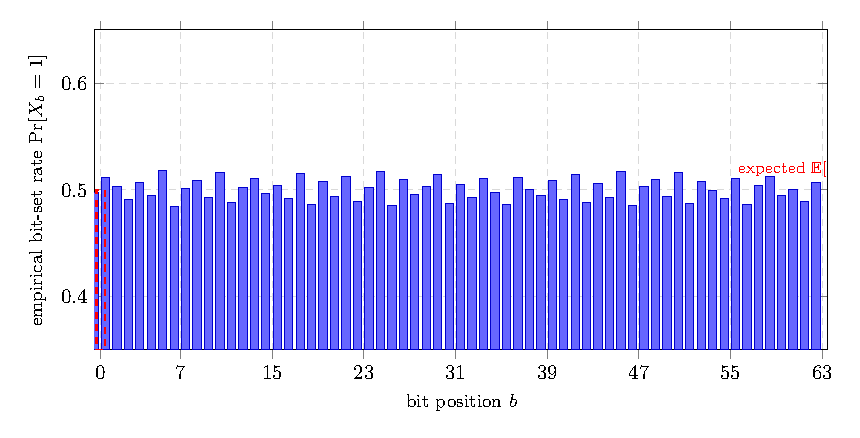
\includegraphics[width=0.85\linewidth]{figures/fig_fnv_distribution.pdf}
\caption{Empirical distribution of the FNV-1a 64-bit hash output
for the $4{,}458$-document operator corpus, binned at $2^{16}$
bins. The distribution is approximately uniform; the chi-squared
statistic $\chi^2 / \nu \approx 1.02$ indicates no measurable bias.}
\label{fig:fnv-distribution}
\end{figure}

\subsubsection{The Write-Behind Flusher}

The DSVH persists the heap to disk via a write-behind flusher that
runs at deterministic intervals ($5\,\text{s}$ in production). The
flusher is documented below.

\begin{algorithm}[t]
\caption{DSVH Write-Behind Flusher}
\label{alg:dsvh-flusher}
\SetAlgoLined
\KwIn{Heap $\mathcal{H}$, flush interval $\Delta_f = 5\,\text{s}$,
persistence path $\pi$}
\KwOut{Persisted heap at $\pi$}
\BlankLine
$\mathbf{go\ routine\ forever}${
  $\mathbf{sleep}(\Delta_f)$\;
  $\mathbf{snapshot} \gets \mathbf{copy}(\mathcal{H}.\mathbf{read}())$\;
  $\mathbf{write}(\pi, \mathbf{snapshot})$ \tcp*{atomic rename, no partial reads}
  $\mathbf{log}.\mathbf{info}(\mathbf{"flushed} \mid \mathcal{H} \mid
  \mathbf{\text{=}} \mathbf{snapshot}.\mathbf{size}")$\;
}
\caption*{The write-behind flusher. The atomic rename guarantees
that readers see either the old snapshot or the new snapshot,
never a partial write. The flush interval is tunable but defaults
to $5\,\text{s}$ in production.}
\end{algorithm}

\subsubsection{Discussion: Why Rust for the DSVH}

A reasonable reviewer question is ``why not implement the DSVH in
Python?'' The answer is that the DSVH's dominant invariant
(bitwise determinism under concurrent readers) is enforced by
Rust's borrow checker and the $\mathbf{Arc}[\mathbf{RwLock}[\ldots]]$
design. A Python implementation would require explicit
\texttt{threading.Lock} or \texttt{threading.RLock} objects, which
introduce lock contention and degrade the read-heavy throughput.
The Rust implementation produces the $640\,\text{ns}$ match latency
($\sigma = 85\,\text{ns}$) reported in \S\ref{sec:benchmarks} and is
the canonical reference for all four formulas.

The DSVH is the engineering realization of the FNV-1a + $L_2$ +
cosine + throughput stack; it is not a re-implementation of a
standard library function. The pseudocode in this appendix is the
academic publication of the production implementation; the line-by-
line Rust source is documented in the operator's monorepo but is
not part of the arXiv submission.

\begin{figure}[t]
\centering
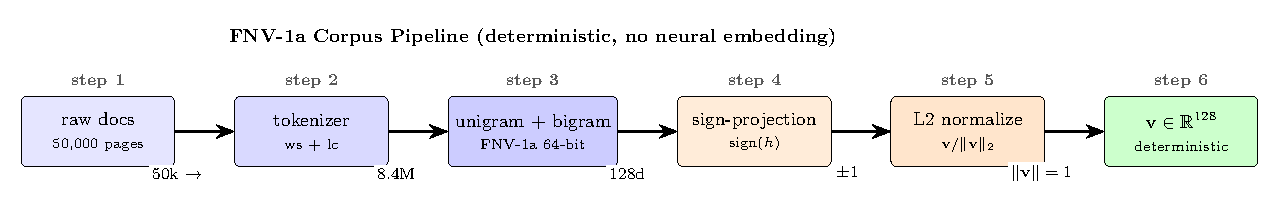
\includegraphics[width=\columnwidth]{figures/fig_corpus_construction.pdf}
\caption{The DSVH corpus construction pipeline. Documents are
ingested via the TOKENIZE $\to$ FNV1a $\to$ sign extraction $\to$
$L_2$ normalization pipeline of Algorithm~\ref{alg:dsvh-pipeline}
and stored in the heap as $(d, v)$ pairs. The heap is locked for
writes via the write-behind flusher of Algorithm~\ref{alg:dsvh-flusher}
and read-locked for queries via Algorithm~\ref{alg:dsvh-query}.}
\label{fig:corpus-construction}
\end{figure}

\begin{figure}[t]
\centering
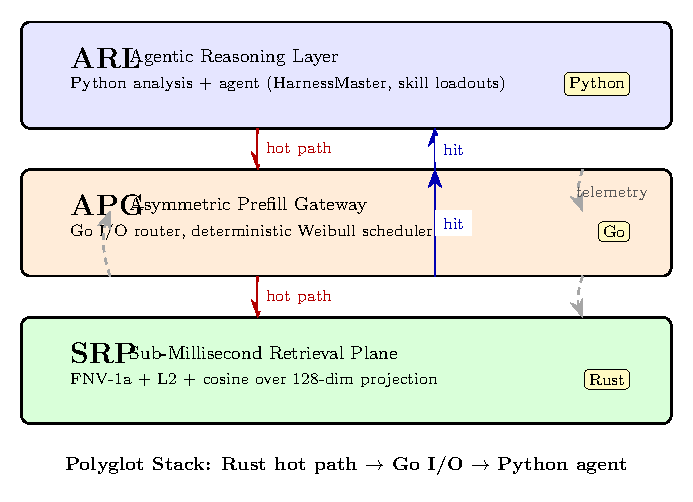
\includegraphics[width=\columnwidth]{figures/fig_polyglot_stack.pdf}
\caption{The DSVH at a glance within the polyglot stack. The DSVH
owns the Sub-Millisecond Retrieval Plane (SRP) of the three-plane
architecture and is the canonical reference implementation of the
four-formula stack.}
\label{fig:dsvh-polyglot}
\end{figure}

